%    minted language=cpp,

\documentclass[pdf,
%8pt, 9pt, 10pt, 11pt, 12pt, 14pt, 17pt, 20pt
serif,
%handout,	% remove overlays
compress,
xcolor=table,
dvipsnames,
spanish,
aspectratio=169]{beamer}

\usepackage[algosection,lined]{algorithm2e}
\usepackage{minted}
\usepackage{tcolorbox}
\tcbuselibrary{minted}

%% Otros
\usepackage{xcolor}
%\usepackage[dvipsnames]{xcolor}

\usepackage[linguistics]{forest}
\forestset{child frame/.style=
    {tikz={\node () [rectangle, red,draw, fit to=children,inner sep = 0pt] {};}}}


%% Encoding, fonts, language
%% Font & Encoding
\usepackage{libertine}
\usepackage[libertine]{newtxmath}
\usepackage[scaled=0.8]{beramono}  % for monospaced font
\usepackage{microtype}		% micro-typographic aspects of the fonts
\usepackage[T1]{fontenc}	% special fonts, e.g. for German umlaute
%% incompabtible with Biblatex
% \usepackage{ucs}
% \usepackage[utf8x]{inputenc}
%% compatible with Biblatex
\usepackage[utf8]{inputenc}



%% Language
%\usepackage[german]{babel}
%\usepackage{german}
\usepackage[english]{babel}


 
\usepackage{graphics}
\usepackage{url}
\usepackage{amsmath,amssymb,amsfonts,marvosym}
\usepackage{ulem}			% to cross out text
\usepackage{subfig}			% to cross out text
\normalem
\usepackage{ragged2e}
\let\raggedright=\RaggedRight
%%%%%%%%%%%%%%%%%%%%%%%%
%   BEAMER SETTINGS    % 
%%%%%%%%%%%%%%%%%%%%%%%%

%\usefonttheme{serif}
%\renewcommand*{\ttdefault}{cmtt}

\definecolor{HHUblue}{HTML}{006AB3}
\setbeamercolor{structure}{fg=HHUblue}

\hypersetup{colorlinks,linkcolor=green,urlcolor=blue}

\setbeamerfont{frametitle}{family=\sffamily}
\setbeamerfont{title}{family=\sffamily}
\setbeamerfont{block title}{family=\sffamily}

%\usetheme{Copenhagen} % Boadilla
\usetheme{Warsaw}
\usecolortheme[rgb={0,0.4,0}]{structure}

\usecolortheme{default}   % beaver
\usefonttheme{default}		% default | professionalfonts | serif | structurebold | structureitalicserif | structuresmallcapsserif
\useinnertheme{default} 	% circles | default | inmargin | rectangles | rounded
\useoutertheme{default}	% default | infolines | miniframes | shadow | sidebar | smoothbars | smoothtree | split | tree

%\setbeamercovered{transparent}				% for transparent overlays
\setbeamercovered{invisible}				% for non-transparent overlays
\setbeamertemplate{navigation symbols}{}	% no navigation symbols
\setbeamertemplate{headline}[default]		% no headline
\setbeamertemplate{footline}[frame number]
\setbeamertemplate{section in toc}[]
\setbeamertemplate{subsection in toc}[]
\setbeamertemplate{itemize items}[square]
\setbeamertemplate{enumerate items}[square]
%\setbeamertemplate{blocks}[default]		% rectangular blocks
%\setbeamersize{text margin left=10pt,text margin right=10pt}

%% Bibliography style (http://tex.stackexchange.com/questions/97615/article-style-bibliography-in-beamer-class)
\setbeamertemplate{frametitle continuation}[from second]
% Now get rid of all the colours
\setbeamercolor*{bibliography entry title}{fg=black}
\setbeamercolor*{bibliography entry author}{fg=black}
\setbeamercolor*{bibliography entry location}{fg=black}
\setbeamercolor*{bibliography entry note}{fg=black}
% and kill the abominable icon
\setbeamertemplate{bibliography item}{\insertbiblabel}  % insert label from bib(la)tex
\AtBeginDocument{
  \renewcommand*{\bibfont}{\scriptsize}
}

%\tikzset{% makes available \only and \alt inside paths
%  only/.code args={<#1>#2}{\only<#1>{\pgfkeysalso{#2}}},
%  alt/.code args={<#1>#2#3}{\alt<#1>{\pgfkeysalso{#2}}{\pgfkeysalso{#3}}}
%}

\setbeamertemplate{footline}
{
  \leavevmode%
  \hbox{%
    \pgfsetfillopacity{0}\begin{beamercolorbox}[wd=.333333\paperwidth,ht=2.25ex,dp=1ex,left]{author in head/foot}%
      \usebeamerfont{author in head/foot}\pgfsetfillopacity{1}\color{gray}\hspace*{2ex}\insertshortauthor~~(\insertshortinstitute)
    \end{beamercolorbox}%
    \pgfsetfillopacity{0}\begin{beamercolorbox}[wd=.333333\paperwidth,ht=2.25ex,dp=1ex,center]{title in head/foot}%
      %\usebeamerfont{title in head/foot}\pgfsetfillopacity{1}\insertshorttitle
    \end{beamercolorbox}%
    \pgfsetfillopacity{0}\begin{beamercolorbox}[wd=.333333\paperwidth,ht=2.25ex,dp=1ex,right]{date in head/foot}%
      \usebeamerfont{date in head/foot}\pgfsetfillopacity{1}\insertshortdate{}\color{gray}\hspace*{2em}
      \insertframenumber{} %/ \inserttotalframenumber
      \hspace*{2ex}
    \end{beamercolorbox}}%
  \vskip0pt%
}


\newcommand{\separationframe}[1]{
\begin{frame}
\frametitle{}

\begin{center}
  \LARGE 
  \settowidth{\stmueTmp}{ #1 }
    \begin{minipage}{\stmueTmp}
    \begin{block}{}
    \begin{center}
    %\usebeamercolor[fg]{frametitle}
    #1
    \end{center}
    \end{block}
    \end{minipage}
\end{center}

\end{frame}
}

\newcommand\framecite[1]{
\vskip-2ex
\hfill #1%
\vskip-3.3ex ~
}

\usepackage[
  hyperref=true,
  url=true,
  natbib=true,  
  %style=bst/biblatex-sp-unified,
  style=ieee,
  %citestyle=\mycitestyle,
  %refsection=chapter,
  maxbibnames=99,
  isbn=false,
  doi=false,
  eprint=false,
  backend=biber,
  %backend=bibtex,
  % sorting=ydnt,  % sort in descending chronological order
  indexing=cite,
  labelnumber,  % for numeric bibliography in beamer
  %toc=bib    % make bibliography appear in toc, incompatible with beamer
]{biblatex}   % bibliography

\addbibresource[datatype=bibtex]{references.bib}

\newcommand{\insertBib}{
  \printbibliography[
    %notkeyword=this
    ] 
}


\usepackage{datetime}
\newdateformat{specialdate}{\twodigit{\THEDAY}-\twodigit{\THEMONTH}-\THEYEAR}
%\newdateformat{specialdate}{\twodigit{\THEDAY}-\THEYEAR}
\date{\specialdate\today}

%%%%%%%%%%%%%%%%%%%%%%%%%%%%%%%%%%%%%%%%%%%%%%%%%%%%%%%%%%%%%%%%%
% HEADER
%%%%%%%%%%%%%%%%%%%%%%%%%%%%%%%%%%%%%%%%%%%%%%%%%%%%%%%%%%%%%%%%%

%\title[\arabic{page} ]{Advanced Computer Graphics}
\title[Arrays]{Kotlin}
% Sin subtitulos
\subtitle[short]{Capture and Pick Image Demo}
% Corchetes: Solo apellidos de los integrantes, Llaves: Los nombres completos!!
\author[-]{Juan Daniel Torres Colorado}
\institute[UPV]{Polytechnic University of Victoria}
\date[]{January-April 2024}
\logo{\pgfimage[width=1cm,height=1cm]{graphics/logo_upv_transparente}}			% Logo on all slides (pdf,png,jpg,eps)
\titlegraphic{
\includegraphics[height=1.5cm]{graphics/logo_upv_transparente} \hfil 
\includegraphics[height=1.8cm]{graphics/kotlin.png}}	% Logo on title slide


%%%%%%%%%%%%%%%%%%%%%%%%%%%%%%%%%%%%%%%%%%%%%%%%%%%%%%%%%%%%%%%%%
% SLIDES
%%%%%%%%%%%%%%%%%%%%%%%%%%%%%%%%%%%%%%%%%%%%%%%%%%%%%%%%%%%%%%%%%

% Configuracion para dibujar AUTOMATAS
\usepackage{tikz}
\usetikzlibrary{automata, positioning, arrows, shapes}

\tikzset{My Arrow Style/.style={single arrow, fill=red!50, anchor=base, align=center,text width=0.35cm, single arrow head extend=0.1cm, single arrow head indent=0.01cm}}
\newcommand{\MyArrow}[2][]{\tikz[baseline] \node [My Arrow Style,#1] {#2};}

\definecolor{naranja}{RGB}{190, 45, 0}
\definecolor{purpura}{RGB}{64, 69, 140}
\definecolor{crema}{RGB}{236, 216, 130}
\definecolor{celeste}{RGB}{207, 219, 253}
\definecolor{tablepurpura}{RGB}{212,214,212}
\definecolor{tablecrema}{RGB}{248,240,208}
\definecolor{tableamarillo}{RGB}{236,216,130}

\tikzset{
    fath/.style={draw, ellipse, fill=crema, draw=purpura, text=purpura, inner sep=2pt},
    none/.style={draw, rectangle, fill=celeste, draw=purpura,               text=purpura, minimum size=1.2em},
    noneLow/.style={draw, rectangle, fill=celeste, draw=purpura,               text=purpura, minimum size=0.7em},
    conn/.style={-, purpura, thick, overlay},
}

\begin{document}
% Diapositiva de títulodiaposi
%\begin{frame}[plain]
%  \titlepage
%\end{frame}

\begin{frame} 
    \vspace{1.5cm}
    \textcolor{naranja}{\huge (2,4) Trees: Very Briefly}

    \vspace{1.5cm}
    \hspace{7cm}
    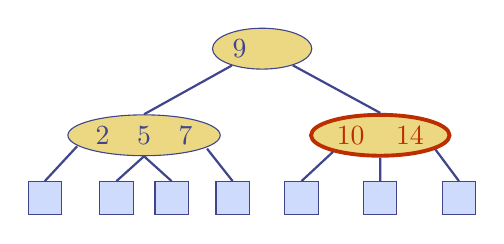
\begin{tikzpicture}[
        level 1/.style={sibling distance=3cm},
        level 2/.style={sibling distance=1cm, level distance=0.8cm},
        level 3/.style={sibling distance=1.3cm, level distance=0.8cm},
        level distance=1.1cm,
        edge from parent/.style={draw=none},
        ]
        \node [fath] (r) {9\hspace{0.4cm}\textcolor{crema}{1}}
            child {
                node [fath] (ch1) {2\hspace{0.35cm}5\hspace{0.35cm}7}
                child [sibling distance=0.84 cm] {node[none] (ch1a) { }}
                child [sibling distance=0.7 cm] {node[none] (ch1b) { }}
                child [sibling distance=0.7 cm] {node[none] (ch1c) { }}
                child [sibling distance=0.75 cm] {node[none] (ch1d) { }}
            }
            child {
                node[fath, draw=naranja, line width=1.4pt, text=naranja] (ch2) {10\hspace{0.4cm}14}
                child {node[none] (ch2a) { }}
                child {node[none] (ch2b) { }}
                child {node[none] (ch2c) { }}
            };

            \draw[conn] (r) -- (ch1.north);
            \draw[conn] (r) -- (ch2.north);

            \draw[conn] (ch1a.north) -- (-2.35, -1.24);
            \draw[conn] (ch1b.north) -- (ch1.south);
            \draw[conn] (ch1c.north) -- (ch1.south);
            \draw[conn] (ch1d.north) -- (-0.7, -1.27);

            \draw[conn] (ch2a.north) -- (0.9, -1.31);
            \draw[conn] (ch2b.north) -- (ch2.south);
            \draw[conn] (ch2c.north) -- (2.2, -1.28);
    \end{tikzpicture}
\end{frame}

\begin{frame}
    \frametitle{Multi-Way Search Tree}
    \begin{itemize} \color{purpura}
        \item[\(\diamondsuit\)] A multi-way search tree is an ordered tree such that
        \begin{itemize} \color{purpura}
            \item Each internal node has at least two children and stores \(\mathbf{\textit{\textbf{d}}} - 1\) key-element items (\(\mathbf{\textit{\textbf{k}}}_\mathbf{\textit{\textbf{i}}}, \mathbf{\textit{\textbf{o}}}_\mathbf{\textit{\textbf{i}}}\)), where \(\mathbf{\textit{\textbf{d}}}\) is the number of children.
    
            \item For a node with children \(\textit{\textbf{v}}_1, \textit{\textbf{v}}_2, \ldots, \textit{\textbf{v}}_\mathbf{\textit{\textbf{d}}}\) storing keys \(\textit{\textbf{k}}_1, \textit{\textbf{k}}_2, \ldots, \textit{\textbf{k}}_\mathbf{\textit{\textbf{d}}}-1\):
            \begin{itemize} \color{purpura}
                \item[\(\diamondsuit\)] keys in the subtree of \(\textit{\textbf{v}}_1\) are less than \(\textit{\textbf{k}}_1\)
                \item[\(\diamondsuit\)] keys in the subtree of \(\textit{\textbf{v}}_i\) are between \(\mathbf{\textit{\textbf{k}}}_{\textbf{\textit{i}}-1}\) and \(\textit{\textbf{k}}_i\) (\(i = 2, \ldots, \mathbf{\textit{\textbf{d}}} - 1\))
                \item[\(\diamondsuit\)] keys in the subtree of \(\textit{\textbf{v}}_\mathbf{\textit{\textbf{d}}}\) are greater than \(\textit{\textbf{k}}_\mathbf{\textit{\textbf{d}}}-1\)
            \end{itemize}
    
            \item The leaves store no items and serve as placeholders
        \end{itemize}
    \end{itemize}

    \vspace{0.5cm}
    \hspace{2cm}
    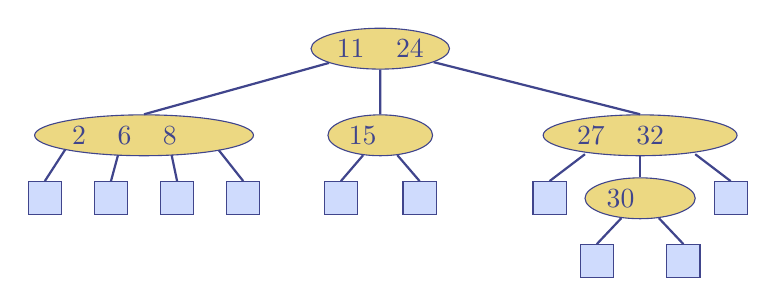
\begin{tikzpicture}[
        level 1/.style={sibling distance=3cm},
        level 2/.style={sibling distance=1cm, level distance=0.8cm},
        level 3/.style={sibling distance=1.1cm, level distance=0.8cm},
        level distance=1.1cm,
        edge from parent/.style={draw=none},
        ]
        \node [fath] (r) {11\hspace{0.4cm}24}
            child {
                node [fath] (ch1) {2\hspace{0.4cm}6\hspace{0.4cm}8\hspace{0.4cm}\textcolor{crema}{.}}
                child [sibling distance=0.84 cm] {node[none] (ch1a) { }}
                child [sibling distance=0.84 cm] {node[none] (ch1b) { }}
                child [sibling distance=0.84 cm] {node[none] (ch1c) { }}
                child [sibling distance=0.84 cm] {node[none] (ch1d) { }}
            }
            child {
                node[fath] (ch2) {15\hspace{0.35cm}\textcolor{crema}{.}}
                child {node[none] (ch2a) { }}
                child {node[none] (ch2b) { }}
            }
            child [sibling distance=3.3 cm] {
                node[fath] (ch3) {27\hspace{0.4cm}32\hspace{0.4cm}\textcolor{crema}{.}}
                child [sibling distance=1.15 cm] {node[none] (ch3a) { }}
                child [sibling distance=1.15 cm] {
                    node[fath] (ch3b) {30\hspace{0.4cm}\textcolor{crema}{.}}
                    child {node[none] (ch3b1) { }}
                    child {node[none] (ch3b2) { }}
                }
                child [sibling distance=1.15 cm] {node[none] (ch3c) { }}
            };
            
        \draw[conn] (r) -- (ch1.north);
        \draw[conn] (r) -- (ch2.north);
        \draw[conn] (r) -- (ch3.north);
        \draw[conn] (-4,-1.28) -- (ch1a.north);
        \draw[conn] (-3.33,-1.35) -- (ch1b.north);
        \draw[conn] (-2.65,-1.35) -- (ch1c.north);   
        \draw[conn] (-2.05,-1.29) -- (ch1d.north);
        \draw[conn] (ch2) -- (ch2a.north);
        \draw[conn] (ch2) -- (ch2b.north);
        \draw[conn] (2.6,-1.34) -- (ch3a.north);
        \draw[conn] (ch3b.north) -- (ch3.south);
        \draw[conn] (4,-1.34) -- (ch3c.north);
        \draw[conn] (ch3b) -- (ch3b1.north);
        \draw[conn] (ch3b) -- (ch3b2.north);
    \end{tikzpicture}
\end{frame}

\begin{frame}
    \frametitle{Multi-Way Inorder Traversal}
    \begin{itemize}
        \color{purpura}
        \item[\(\diamondsuit\)] We can extend the notion of inorder traversal from binary trees to multi-way search trees
        \item[\(\diamondsuit\)] Namely, we visit item \((\mathbf{\textit{\textbf{k}}}_{\mathbf{\textit{\textbf{i}}}}, \mathbf{\textit{\textbf{o}}}_{\mathbf{\textit{\textbf{i}}}})\) of node \(\mathbf{\textbf{v}}\) between the recursive traversals of the subtrees of \(\mathbf{\textit{\textbf{v}}}_{\mathbf{\textit{\textbf{i}}}}\) and \(\mathbf{\textit{\textbf{v}}}_{\mathbf{\textit{\textbf{i}}}+1}\)
    
        \item[\(\diamondsuit\)] An inorder traversal of a multi-way search tree visits the keys in increasing order
    \end{itemize}

    \vspace{0.5cm}
    \hspace{2cm}
    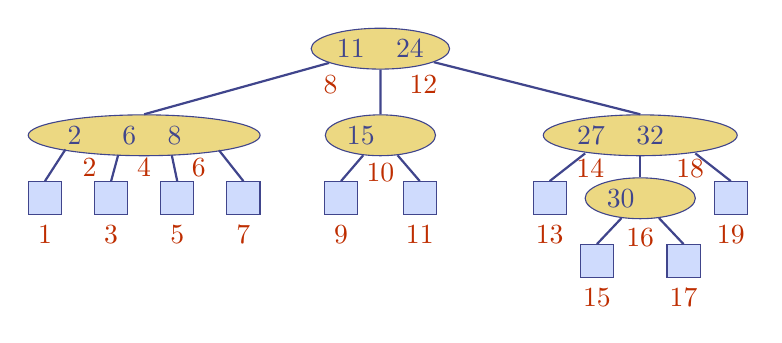
\begin{tikzpicture}[
        level 1/.style={sibling distance=3cm},
        level 2/.style={sibling distance=1cm, level distance=0.8cm},
        level 3/.style={sibling distance=1.1cm, level distance=0.8cm},
        level distance=1.1cm,
        edge from parent/.style={draw=none},
        ]
        \node [fath] (r) {11\hspace{0.4cm}24}
            child {
                node [fath] (ch1) {2 \hspace{0.4cm}6\hspace{0.4cm}8\hspace{0.4cm}\textcolor{crema}{.}}
                child [sibling distance=0.84 cm] {node[none] (ch1a) { }}
                child [sibling distance=0.84 cm] {node[none] (ch1b) { }}
                child [sibling distance=0.84 cm] {node[none] (ch1c) { }}
                child [sibling distance=0.84 cm] {node[none] (ch1d) { }}
            }
            child {
                node[fath] (ch2) {15\hspace{0.4cm}\textcolor{crema}{.}}
                child {node[none] (ch2a) { }}
                child {node[none] (ch2b) { }}
            }
            child [sibling distance=3.3 cm] {
                node[fath] (ch3) {27\hspace{0.4cm}32\hspace{0.4cm}\textcolor{crema}{.}}
                child [sibling distance=1.15 cm] {node[none] (ch3a) { }}
                child [sibling distance=1.15 cm] {
                    node[fath] (ch3b) {30\hspace{0.4cm}\textcolor{crema}{.}}
                    child {node[none] (ch3b1) { }}
                    child {node[none] (ch3b2) { }}
                }
                child [sibling distance=1.15 cm] {node[none] (ch3c) { }}
            };

        \node[text=naranja] at (0, -0.45) {8\hspace{0.4cm} \hspace{0.4cm}12};

        \node[text=naranja] at (-3,-1.51) {2\hspace{0.4cm} 4 \hspace{0.4cm}6};
        \node[text=naranja, below=0cm of ch1a] {1};
        \node[text=naranja, below=0cm of ch1b] {3};
        \node[text=naranja, below=0cm of ch1c] {5};
        \node[text=naranja, below=0cm of ch1d] {7};
        
        \node[text=naranja] at (0, -1.57) {10};
        \node[text=naranja, below=0cm of ch2a] {9};
        \node[text=naranja, below=0cm of ch2b] {11};

        \node[text=naranja] at (3.3,-1.52) {14\hspace{0.4cm} \hspace{0.4cm}18};
        \node[text=naranja, below=0cm of ch3a] {13};
        \node[text=naranja] at (3.3,-2.4) {16};
        \node[text=naranja, below=0cm of ch3b1] {15};
        \node[text=naranja, below=0cm of ch3b2] {17};
        \node[text=naranja, below=0cm of ch3c] {19};
                
        \draw[conn] (r) -- (ch1.north);
        \draw[conn] (r) -- (ch2.north);
        \draw[conn] (r) -- (ch3.north);
        \draw[conn] (-4,-1.28) -- (ch1a.north);
        \draw[conn] (-3.33,-1.35) -- (ch1b.north);
        \draw[conn] (-2.65,-1.35) -- (ch1c.north);   
        \draw[conn] (-2.05,-1.29) -- (ch1d.north);
        \draw[conn] (ch2) -- (ch2a.north);
        \draw[conn] (ch2) -- (ch2b.north);
        \draw[conn] (2.6,-1.33) -- (ch3a.north);
        \draw[conn] (ch3b.north) -- (ch3.south);
        \draw[conn] (4,-1.33) -- (ch3c.north);
        \draw[conn] (ch3b) -- (ch3b1.north);
        \draw[conn] (ch3b) -- (ch3b2.north);
    \end{tikzpicture}
\end{frame}

\begin{frame} {Multi-Way Searching}
    \begin{itemize} \color{purpura}
        \item[\(\diamondsuit\)] Similar to search in a binary search tree
        \item[\(\diamondsuit\)] At each internal node with children \(\textit{\textbf{v}}_1\ \textit{\textbf{v}}_2\ ... \textit{\textbf{v}}_{\textit{\textbf{d}}}\) and keys \(\textit{\textbf{k}}_1\ \textit{\textbf{k}}_2\ ... \textit{\textbf{k}}_{\textit{\textbf{d}}-1}\)
        \begin{itemize} \color{purpura}
            \item \(\mathbf{\textit{\textbf{k}}} = \textit{\textbf{k}}_{\textit{\textbf{i}}}\) (\(\textbf{\textit{i}} = 1, ..., \textbf{\textit{d}} - 1\)): the search terminates successfully
    
            \item \(\mathbf{\textit{\textbf{k}}} < \textit{\textbf{k}}_1\): we continue the search in child \(\textit{\textbf{v}}_1\)
    
            \item \(\textit{\textbf{k}}_{\textit{\textbf{i}}-1} < \mathbf{\textit{\textbf{k}}} < \textit{\textbf{k}}_{\textit{\textbf{i}}}\) (\(\textbf{\textit{i}} = 2, ..., \textbf{\textit{d}} - 1\)): we continue the search in child \(\textit{\textbf{v}}_{\textit{\textbf{i}}}\)
    
            \item \(\mathbf{\textit{\textbf{k}}} > \textit{\textbf{k}}_{\textit{\textbf{d}}-1}\): we continue the search in child \(\textit{\textbf{v}}_{\textit{\textbf{d}}}\)
        \end{itemize}
        
        \item[\(\diamondsuit\)] Reaching an external node terminates the search unsuccessfully
        \item[\(\diamondsuit\)] Example: search for 30
    \end{itemize}

    \vspace{0.5cm}
    \hspace{2cm}
    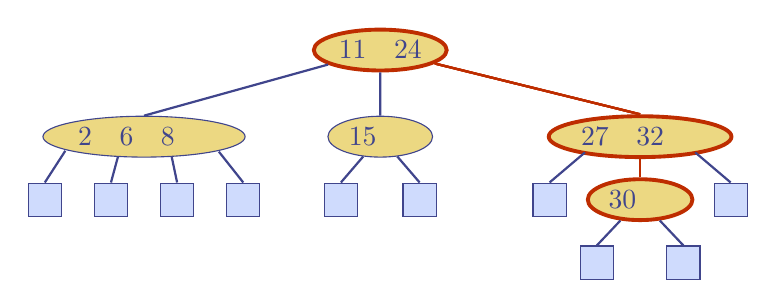
\begin{tikzpicture}[
        level 1/.style={sibling distance=3cm},
        level 2/.style={sibling distance=1cm, level distance=0.8cm},
        level 3/.style={sibling distance=1.1cm, level distance=0.8cm},
        level distance=1.1cm,
        edge from parent/.style={draw=none},
        ]
        \node [fath, draw=naranja, line width=1.4pt] (r) {11\hspace{0.35cm}24}
            child {
                node [fath] (ch1) {2\hspace{0.35cm}6\hspace{0.35cm}8\hspace{0.35cm}\textcolor{crema}{.}}
                child [sibling distance=0.84 cm] {node[none] (ch1a) { }}
                child [sibling distance=0.84 cm] {node[none] (ch1b) { }}
                child [sibling distance=0.84 cm] {node[none] (ch1c) { }}
                child [sibling distance=0.84 cm] {node[none] (ch1d) { }}
            }
            child {
                node[fath] (ch2) {15\hspace{0.35cm}\textcolor{crema}{.}}
                child {node[none] (ch2a) { }}
                child {node[none] (ch2b) { }}
            }
            child [sibling distance=3.3 cm] {
                node[fath, draw=naranja, line width=1.4pt] (ch3) {27\hspace{0.35cm}32\hspace{0.35cm}\textcolor{crema}{.}}
                child [sibling distance=1.15 cm] {node[none] (ch3a) { }}
                child [sibling distance=1.15 cm] {
                    node[fath, draw=naranja, line width=1.4pt] (ch3b) {30\hspace{0.35cm}\textcolor{crema}{.}}
                    child {node[none] (ch3b1) { }}
                    child {node[none] (ch3b2) { }}
                }
                child [sibling distance=1.15 cm] {node[none] (ch3c) { }}
            };
            
        \draw[conn] (r) -- (ch1.north);
        \draw[conn] (r) -- (ch2.north);
        \draw[conn, naranja] (r) -- (ch3.north);
        \draw[conn, naranja] (r) -- (ch3.north);
        \draw[conn, naranja] (r) -- (ch3.north);
        \draw[conn, naranja] (r) -- (ch3.north);
        \draw[conn] (-4,-1.28) -- (ch1a.north);
        \draw[conn] (-3.33,-1.35) -- (ch1b.north);
        \draw[conn] (-2.65,-1.35) -- (ch1c.north);   
        \draw[conn] (-2.05,-1.29) -- (ch1d.north);
        \draw[conn] (ch2) -- (ch2a.north);
        \draw[conn] (ch2) -- (ch2b.north);
        \draw[conn] (2.6,-1.3) -- (ch3a.north);
        \draw[conn, naranja] (ch3b.north) -- (ch3.south);
        \draw[conn, naranja] (ch3b.north) -- (ch3.south);
        \draw[conn, naranja] (ch3b.north) -- (ch3.south);
        \draw[conn, naranja] (ch3b.north) -- (ch3.south);
        \draw[conn] (4,-1.3) -- (ch3c.north);
        \draw[conn] (ch3b) -- (ch3b1.north);
        \draw[conn] (ch3b) -- (ch3b2.north);
    \end{tikzpicture}
\end{frame}

\begin{frame}
    \frametitle{(2,4) Trees}
    \begin{itemize} \color{purpura}
        \item[\(\diamondsuit\)]A (2,4) tree (also called 2-4 tree or 2-3-4 tree) is a multi-way search with the following properties
        \begin{itemize} \color{purpura}
            \item \textcolor{naranja}{Node-Size Property}: every internal node has at most four children (i.e., three keys)
            \item \textcolor{naranja}{Depth Property}: all the external nodes have the same depth
        \end{itemize}

        \item[\(\diamondsuit\)]Depending on the \textcolor{Red}{number of children}, an internal node of a (2,4) tree is called a 2-node, 3-node or 4-node

        \vspace{0.5cm}
        \hspace{1cm}
        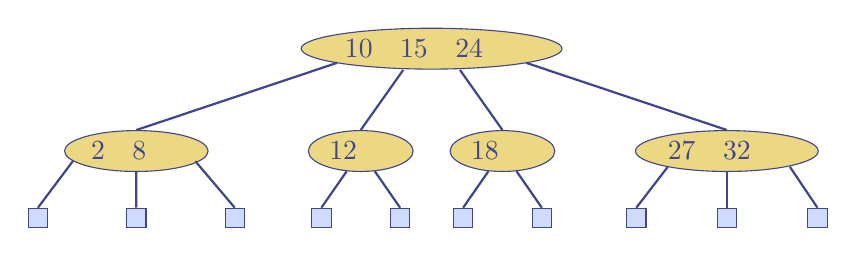
\begin{tikzpicture}[
            level 1/.style={level distance=1.3cm},
            level 2/.style={sibling distance=1cm, level distance=0.85cm},
            edge from parent/.style={draw=none},
            ]
            \node [fath] (r) {10\hspace{0.35cm}15\hspace{0.35cm}24\hspace{0.35cm}\textcolor{crema}{.}}
                child [sibling distance=2.5 cm] {
                    node [fath] (ch1) {2\hspace{0.35cm}8\hspace{0.35cm}\textcolor{crema}{.}}
                    child [sibling distance=1.25cm] {node[noneLow] (ch1a) { }}
                    child [sibling distance=1.25cm] {node[noneLow] (ch1b) { }}
                    child [sibling distance=1.25cm] {node[noneLow] (ch1c) { }}
                }
                child [sibling distance= 1.8 cm] {
                    node[fath] (ch2) {12\hspace{0.35cm}\textcolor{crema}{.}}
                    child {node[noneLow] (ch2a) { }}
                    child {node[noneLow] (ch2b) { }}
                }
                child [sibling distance= 1.8 cm] {
                    node[fath] (ch3) {18\hspace{0.35cm}\textcolor{crema}{.}}
                    child {node[noneLow] (ch3a) { }}
                    child {node[noneLow] (ch3b) { }}
                }
                child [sibling distance=2.5 cm] {
                    node[fath] (ch4) {27\hspace{0.35cm}32\hspace{0.35cm}\textcolor{crema}{.}}
                    child [sibling distance=1.15 cm] {node[noneLow] (ch4a) { }}
                    child [sibling distance=1.15 cm] {node[noneLow] (ch4b) { }}
                    child [sibling distance=1.15 cm] {node[noneLow] (ch4c) { }}
                };

                \draw[conn] (-1.2,-0.18) -- (ch1.north);
                \draw[conn] (-0.36, -0.27) -- (ch2.north);
                \draw[conn] (0.36, -0.27) -- (ch3.north);
                \draw[conn] (1.2,-0.18) -- (ch4.north);

                \draw[conn] (-4.55, -1.42) -- (ch1a.north);
                \draw[conn] (ch1.south) -- (ch1b.north);
                \draw[conn] (-3, -1.43) -- (ch1c.north);

                \draw[conn] (ch2) -- (ch2a.north);
                \draw[conn] (ch2) -- (ch2b.north);

                \draw[conn] (ch3) -- (ch3a.north);
                \draw[conn] (ch3) -- (ch3b.north);

                \draw[conn] (3, -1.5) -- (ch4a.north);
                \draw[conn] (ch4.south) -- (ch4b.north);
                \draw[conn] (4.55, -1.5) -- (ch4c.north);
        \end{tikzpicture}
        \vspace{0.8cm}
        \item[\(\diamondsuit\)] \textcolor{red}{(Question)} Why not like the ”height-balancing property” of AVL trees?
    \end{itemize}    
\end{frame}

\begin{frame}
    \frametitle{Height of a (2,4) Tree}
    \begin{itemize} \color{purpura}
        \item[\(\diamondsuit\)] \textcolor{naranja}{Theorem:} A (2,4) tree storing \textbf{\textit{n}} items has height \textbf{\textit{O}}(log \textbf{\textit{n}})
        \vspace{0.5cm}
        \item[\(\diamondsuit\)]Proof: Obvious :)
    \end{itemize}

    \vspace{1.4cm}
    \hspace{1cm}
    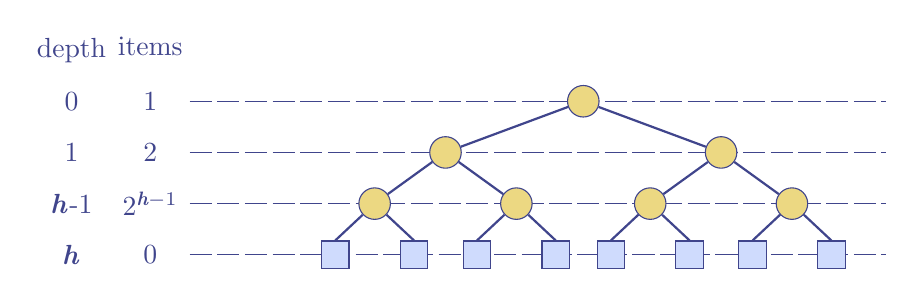
\begin{tikzpicture}[
            level 1/.style={sibling distance=3.5cm},
            level 2/.style={sibling distance=1.8cm},
            level 3/.style={sibling distance=1cm},
            edge from parent/.style={draw=none},
            level distance=0.65cm
            ]

            \node[text=purpura] at (-6.5, 0.64) {depth};
            \node[text=purpura] at (-5.5, 0.7) {items};

            \draw[draw, dash pattern=on 8pt off 2pt, purpura] (-5,0) -- (3.85,0);
            \draw[draw, dash pattern=on 8pt off 2pt, purpura] (-5,-0.65) -- (3.85,-0.65);
            \draw[draw, dash pattern=on 8pt off 2pt, purpura] (-5,-1.3) -- (3.85,-1.3);
            \draw[draw, dash pattern=on 8pt off 2pt, purpura] (-5,-1.95) -- (3.85,-1.95);

            \node [fath, minimum size=0.4cm] (r) { }
                child {
                    node [fath, minimum size=0.4cm] (ch1) { }
                    child {
                        node[fath, minimum size=0.4cm] (ch1a) { }
                        child{node[noneLow, minimum size=0.35cm] (ch1a1) { }}
                        child{node[noneLow, minimum size=0.35cm] (ch1a2) { }}
                    }
                    child {
                        node[fath, minimum size=0.4cm] (ch1b) { }
                        child{node[noneLow, minimum size=0.35cm] (ch1b1) { }}
                        child{node[noneLow, minimum size=0.35cm] (ch1b2) { }}
                    }
                }
                child {
                    node [fath, minimum size=0.4cm] (ch2) { }
                    child {
                        node[fath, minimum size=0.4cm] (ch2a) { }
                        child{node[noneLow, minimum size=0.35cm] (ch2a1) { }}
                        child{node[noneLow, minimum size=0.35cm] (ch2a2) { }}
                    }
                    child {
                        node[fath, minimum size=0.4cm] (ch2b) { }
                        child{node[noneLow, minimum size=0.35cm] (ch2b1) { }}
                        child{node[noneLow, minimum size=0.35cm] (ch2b2) { }}
                    }
                };            
                
            \node[text=purpura] (l1a) at (-6.5, 0) {0};
            \node[text=purpura] (l2a) at (-6.5, -0.65) {1};
            \node[text=purpura] (l3a) at (-6.5, -1.3) {\textbf{\textit{h}}-1};
            \node[text=purpura] (l4a) at (-6.5, -1.95) {\textbf{\textit{h}}};
            \node[text=purpura] (l1b) at (-5.5, 0) {1};
            \node[text=purpura] (l2b) at (-5.5, -0.65) {2};
            \node[text=purpura] (l3b) at (-5.5, -1.3) {\(2^{\mathbf{\textit{\textbf{h}}}-1}\)};
            \node[text=purpura] (l4b) at (-5.5, -1.95) {0};
            
            \draw[conn] (ch1) -- (r);
            \draw[conn] (ch2) -- (r);
            \draw[conn] (ch1a) -- (ch1);
            \draw[conn] (ch1b) -- (ch1);
            \draw[conn] (ch2a) -- (ch2);
            \draw[conn] (ch2b) -- (ch2);
            \draw[conn] (ch1a1.north) -- (ch1a);
            \draw[conn] (ch1a2.north) -- (ch1a);
            \draw[conn] (ch1b1.north) -- (ch1b);
            \draw[conn] (ch1b2.north) -- (ch1b);
            \draw[conn] (ch2a1.north) -- (ch2a);
            \draw[conn] (ch2a2.north) -- (ch2a);
            \draw[conn] (ch2b1.north) -- (ch2b);
            \draw[conn] (ch2b2.north) -- (ch2b);
        \end{tikzpicture}
\end{frame}

\begin{frame}
    \frametitle{Insertion}
    \begin{itemize}
    \color{purpura}
        \item[\(\diamondsuit\)] Insert a new item (\(\mathbf{\textit{\textbf{k}}}, \mathbf{\textit{\textbf{o}}}\)) at the parent \(\mathbf{\textit{\textbf{v}}}\) of the leaf reached by searching for \(\mathbf{\textit{\textbf{k}}}\)
        \begin{itemize}
            \color{purpura}
            \item We preserve the depth property but 
            \item We may cause an \textcolor{naranja}{overflow} (i.e., node \(\mathbf{\textit{\textbf{v}}}\) may become a 5-node)
        \end{itemize}
        \vspace{0.3cm}
        \item[\(\diamondsuit\)] Example: inserting key 30 causes an overflow
    \end{itemize}

    \vspace{0.15cm}
    
    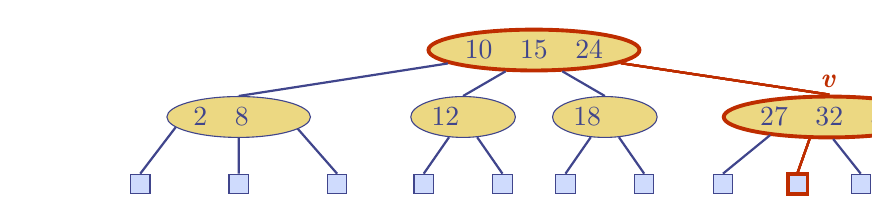
\begin{tikzpicture}[
        level 1/.style={level distance=0.85cm},
        level 2/.style={sibling distance=1cm, level distance=0.85cm},
        edge from parent/.style={draw=none},
        ]
        
        \hspace{1.3cm}
        \node [fath, draw=naranja, line width=1.4pt] (r) {10\hspace{0.35cm}15\hspace{0.35cm}24}
            child [sibling distance=2.5 cm] {
                node [fath] (ch1) {2\hspace{0.35cm}8\hspace{0.35cm}\textcolor{crema}{.}}
                child [sibling distance=1.25cm] {node[noneLow] (ch1a) { }}
                child [sibling distance=1.25cm] {node[noneLow] (ch1b) { }}
                child [sibling distance=1.25cm] {node[noneLow] (ch1c) { }}
            }
            child [sibling distance= 1.8 cm] {
                node[fath] (ch2) {12\hspace{0.35cm}\textcolor{crema}{.}}
                child {node[noneLow] (ch2a) { }}
                child {node[noneLow] (ch2b) { }}
            }
            child [sibling distance= 1.8 cm] {
                node[fath] (ch3) {18\hspace{0.35cm}\textcolor{crema}{.}}
                child {node[noneLow] (ch3a) { }}
                child {node[noneLow] (ch3b) { }}
            }
            child [sibling distance=2.5 cm] {
                node[fath, draw=naranja, line width=1.4pt] (ch4) {27\hspace{0.35cm}32\hspace{0.35cm}35}
                child [sibling distance=0.9cm] {node[noneLow] (ch4a) { }}
                child [sibling distance=0.8cm] {node[noneLow, draw=naranja, line width=1.4pt] (ch4n) { }}
                child [sibling distance=0.8cm] {node[noneLow] (ch4b) { }}
                child [sibling distance=0.9cm] {node[noneLow] (ch4c) { }}
            };

            \draw[conn] (r) -- (ch1.north);
            \draw[conn] (-0.36, -0.27) -- (ch2.north);
            \draw[conn] (0.36, -0.27) -- (ch3.north);
            \draw[conn, naranja] (r) -- (ch4.north);
            \draw[conn, naranja] (r) -- (ch4.north);
            \draw[conn, naranja] (r) -- (ch4.north);
            \draw[conn, naranja] (r) -- (ch4.north);
            \draw[conn, naranja] (r) -- (ch4.north);

            \node[text=naranja, above=0.25cm] (txt1) at (ch4) {\textbf{\textit{v}}};

            \draw[conn] (-4.55, -0.98) -- (ch1a.north);
            \draw[conn] (ch1.south) -- (ch1b.north);
            \draw[conn] (-3, -1) -- (ch1c.north);

            \draw[conn] (ch2) -- (ch2a.north);
            \draw[conn] (ch2) -- (ch2b.north);

            \draw[conn] (ch3) -- (ch3a.north);
            \draw[conn] (ch3) -- (ch3b.north);

            \draw[conn] (3, -1.08) -- (ch4a.north);
            \draw[conn] (3.8, -1.13) -- (ch4b.north);
            \draw[conn, naranja] (3.5, -1.13) -- (ch4n.north);
            \draw[conn, naranja] (3.5, -1.13) -- (ch4n.north);
            \draw[conn, naranja] (3.5, -1.13) -- (ch4n.north);
            \draw[conn, naranja] (3.5, -1.13) -- (ch4n.north);
            \draw[conn, naranja] (3.5, -1.13) -- (ch4n.north);
            \draw[conn] (4.75, -1.05) -- (ch4c.north);
    \end{tikzpicture}

    \hspace{6.13cm}
    \MyArrow[fill=naranja!0, draw=naranja, thick, rotate=270]{} 

    \hspace{1.3cm}
    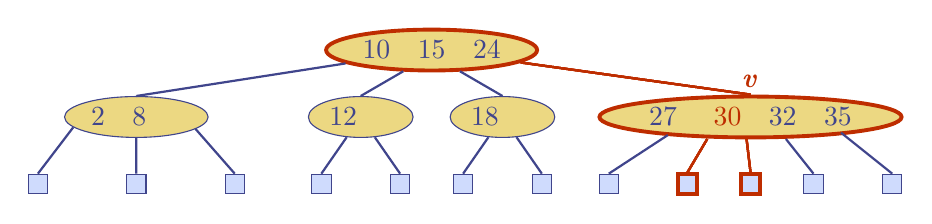
\begin{tikzpicture}[
        level 1/.style={level distance=0.85cm},
        level 2/.style={sibling distance=1cm, level distance=0.85cm},
        edge from parent/.style={draw=none},
        ]
        \node [fath, draw=naranja, line width=1.4pt] (r) {10\hspace{0.35cm}15\hspace{0.35cm}24}
            child [sibling distance=2.5 cm] {
                node [fath] (ch1) {2\hspace{0.35cm}8\hspace{0.35cm}\textcolor{crema}{.}}
                child [sibling distance=1.25cm] {node[noneLow] (ch1a) { }}
                child [sibling distance=1.25cm] {node[noneLow] (ch1b) { }}
                child [sibling distance=1.25cm] {node[noneLow] (ch1c) { }}
            }
            child [sibling distance= 1.8 cm] {
                node[fath] (ch2) {12\hspace{0.35cm}\textcolor{crema}{.}}
                child {node[noneLow] (ch2a) { }}
                child {node[noneLow] (ch2b) { }}
            }
            child [sibling distance= 1.8 cm] {
                node[fath] (ch3) {18\hspace{0.35cm}\textcolor{crema}{.}}
                child {node[noneLow] (ch3a) { }}
                child {node[noneLow] (ch3b) { }}
            }
            child [sibling distance=2.7 cm] {
                node[fath, draw=naranja, line width=1.4pt] (ch4) {27 \hspace{0.35cm}\textcolor{naranja}{30}\hspace{0.35cm}32\hspace{0.35cm}35}
                child [sibling distance=0.9cm] {node[noneLow] (ch4a) { }}
                child [sibling distance=0.8cm] {node[noneLow, draw=naranja, line width=1.4pt] (ch4n) { }}
                child [sibling distance=0.8cm] {node[noneLow, draw=naranja, line width=1.4pt] (ch4m) { }}
                child [sibling distance=0.8cm] {node[noneLow] (ch4b) { }}
                child [sibling distance=0.9cm] {node[noneLow] (ch4c) { }}
            };

            \draw[conn] (r) -- (ch1.north);
            \draw[conn] (-0.36, -0.27) -- (ch2.north);
            \draw[conn] (0.36, -0.27) -- (ch3.north);
            \draw[conn, naranja] (r) -- (ch4.north);
            \draw[conn, naranja] (r) -- (ch4.north);
            \draw[conn, naranja] (r) -- (ch4.north);
            \draw[conn, naranja] (r) -- (ch4.north);
            \draw[conn, naranja] (r) -- (ch4.north);

            \node[text=naranja, above=0.25cm] (txt1) at (ch4) {\textbf{\textit{v}}};

            \draw[conn] (-4.55, -0.98) -- (ch1a.north);
            \draw[conn] (ch1.south) -- (ch1b.north);
            \draw[conn] (-3, -1) -- (ch1c.north);

            \draw[conn] (ch2) -- (ch2a.north);
            \draw[conn] (ch2) -- (ch2b.north);

            \draw[conn] (ch3) -- (ch3a.north);
            \draw[conn] (ch3) -- (ch3b.north);

            \draw[conn] (3, -1.08) -- (ch4a.north);
            \draw[conn] (4.5, -1.13) -- (ch4b.north);
            \draw[conn, naranja] (3.5, -1.13) -- (ch4n.north);
            \draw[conn, naranja] (3.5, -1.13) -- (ch4n.north);
            \draw[conn, naranja] (3.5, -1.13) -- (ch4n.north);
            \draw[conn, naranja] (3.5, -1.13) -- (ch4n.north);
            \draw[conn, naranja] (3.5, -1.13) -- (ch4n.north);
            \draw[conn, naranja] (4, -1.13) -- (ch4m.north);
            \draw[conn, naranja] (4, -1.13) -- (ch4m.north);
            \draw[conn, naranja] (4, -1.13) -- (ch4m.north);
            \draw[conn, naranja] (4, -1.13) -- (ch4m.north);
            \draw[conn, naranja] (4, -1.13) -- (ch4m.north);
            \draw[conn] (5.2, -1.05) -- (ch4c.north);
    \end{tikzpicture}
\end{frame}

\begin{frame}
    \frametitle{Overflow and Split}
    \begin{itemize}
    \color{purpura}
        \item[\(\diamondsuit\)] We handle an \textcolor{naranja}{overflow} at a 5-node \(v\) with a \textcolor{naranja}{split operation}:
        \begin{itemize}
            \color{purpura}
            \item let \(\textit{\textbf{v}}_1, \ldots, \textit{\textbf{v}}_5\) be the children of \(\textbf{\textit{v}}\) and  \(\textit{\textbf{k}}_1, \ldots, \textit{\textbf{k}}_4\) be the keys of \(\textbf{\textit{v}}\)
    
            \item node \(v\) is replaced by nodes \(\textbf{\textit{v'}}\) and \(\textbf{\textit{v''}}\)
            \begin{itemize}
                \color{purpura}
                \item[\(\diamondsuit\)] \(\textbf{\textit{v'}}\) is a 3-node with keys \(\textit{\textbf{k}}_1, \textit{\textbf{k}}_2\) and children \(\textit{\textbf{v}}_1, \textit{\textbf{v}}_2, \textit{\textbf{v}}_3\)
    
                \item[\(\diamondsuit\)] \(\textbf{\textit{v''}}\) is a 2-node with key \(\textit{\textbf{k}}_4\) and children \(\textit{\textbf{v}}_4, \textit{\textbf{v}}_5\)
            \end{itemize}
    
            \item key \(\textit{\textbf{k}}_3\) is inserted into the parent \(\textbf{\textit{u}}\) of \(\textbf{\textit{v}}\) (a new root may be created)
        \end{itemize}
            
        \item[\(\diamondsuit\)] The overflow may propagate to the parent node \(\textbf{\textit{u}}\)
    \end{itemize}

    \begin{minipage}{0.43\linewidth}
         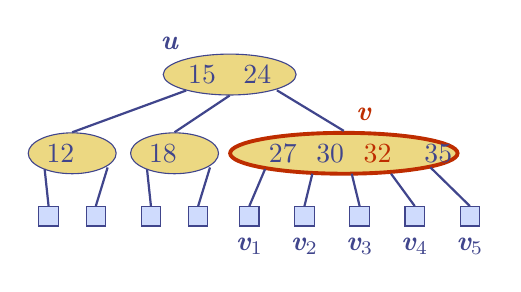
\begin{tikzpicture}[
        level 1/.style={level distance=0.85cm},
        level 2/.style={sibling distance=0.7cm, level distance=0.85cm},
        edge from parent/.style={draw=none},
        ]
        
        \node [purpura] (txt1) at (-0.75,0.4) {\textbf{\textit{u}}};
        \node [fath] (r) {15\hspace{0.35cm}24};
        
        \node [fath] (ch1) at (-2,-1) {12\hspace{0.2cm}\textcolor{crema}{.}};
        \node [noneLow] (ch1a) at (-2.3,-1.8) { };
        \node [noneLow] (ch1b) at (-1.7,-1.8) { };
        
        \node [fath] (ch2) at (-0.7,-1) {18\hspace{0.2cm}\textcolor{crema}{.}};
        \node [noneLow] (ch2a) at (-1,-1.8) { };
        \node [noneLow] (ch2b) at (-0.4,-1.8) { };

        \node [fath, draw=naranja, line width=1.4pt] (ch3) at (1.45,-1) {27\hspace{0.25cm}30\hspace{0.25cm}\textcolor{naranja}{32}\hspace{0.25cm}\textcolor{crema}{.}};
        \node [purpura] (txt2) at (1.7,-0.5) {\textbf{\textit{\textcolor{naranja}{v}}}};
        \node [purpura] (num) at (2.65,-1) {35};
        \node [noneLow] (ch3a) at (0.25,-1.8) {\hspace{0.2cm}};
        \node [noneLow] (ch3b) at (0.95,-1.8) {\hspace{0.2cm}};
        \node [noneLow] (ch3c) at (1.65,-1.8) {\hspace{0.2cm}};
        \node [noneLow] (ch3d) at (2.35,-1.8) {\hspace{0.2cm}};
        \node [noneLow] (ch3e) at (3.05,-1.8) {\hspace{0.2cm}};

        \node [purpura, below=0.15cm] (v1) at (ch3a){\(\textit{\textbf{v}}_1\)};
        \node [purpura, below=0.15cm] (v2) at (ch3b){\(\textit{\textbf{v}}_2\)};
        \node [purpura, below=0.15cm] (v3) at (ch3c){\(\textit{\textbf{v}}_3\)};
        \node [purpura, below=0.15cm] (v4) at (ch3d){\(\textit{\textbf{v}}_4\)};
        \node [purpura, below=0.15cm] (v5) at (ch3e){\(\textit{\textbf{v}}_5\)};

        \draw [conn] (ch1.north) -- (r);
        \draw [conn] (ch2.north) -- (r.south);
        \draw [conn] (ch3.north) -- (0.6,-0.2);

        \draw [conn] (ch1a.north) -- (-2.35,-1.2);
        \draw [conn] (ch1b.north) -- (-1.55,-1.18);

        \draw [conn] (ch2a.north) -- (-1.05,-1.2);
        \draw [conn] (ch2b.north) -- (-0.25,-1.18);

        \draw [conn] (ch3a.north) -- (0.45,-1.2);
        \draw [conn] (ch3b.north) -- (1.05,-1.26);
        \draw [conn] (ch3c.north) -- (1.55,-1.26);
        \draw [conn] (ch3d.north) -- (2.05,-1.26);
        \draw [conn] (ch3e.north) -- (2.55,-1.18);
    \end{tikzpicture} 
    \end{minipage}%
    \begin{minipage}{0.03\linewidth}
        \MyArrow[fill=naranja!0, draw=naranja, thick]{}
    \end{minipage}%
    \begin{minipage}{0.05\linewidth}
        \hspace{0.2cm}
    \end{minipage}%
    \begin{minipage}{0.45\linewidth}
         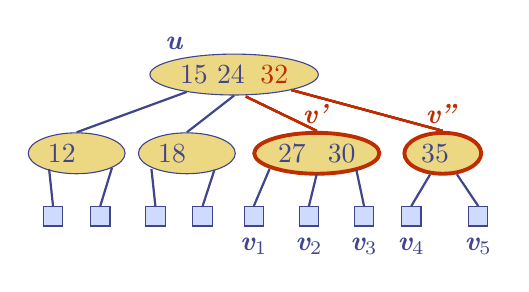
\begin{tikzpicture}[
        level 1/.style={level distance=0.85cm},
        level 2/.style={sibling distance=0.7cm, level distance=0.85cm},
        edge from parent/.style={draw=none},
        ]
        
        \node [purpura] (txt1) at (-0.75,0.4) {\textbf{\textit{u}}};
        \node [fath] (r) {15 24\hspace{0.2cm}\textcolor{naranja}{32}};
        
        \node [fath] (ch1) at (-2,-1) {12\hspace{0.28cm}\textcolor{crema}{.}};
        \node [noneLow] (ch1a) at (-2.3,-1.8) { };
        \node [noneLow] (ch1b) at (-1.7,-1.8) { };
        
        \node [fath] (ch2) at (-0.6,-1) {18\hspace{0.28cm}\textcolor{crema}{.}};
        \node [noneLow] (ch2a) at (-1,-1.8) { };
        \node [noneLow] (ch2b) at (-0.4,-1.8) { };

        \node [naranja] (txt2) at (1.05,-0.5) {\textbf{\textit{v'}}};
        \node [fath, draw=naranja, line width=1.4pt] (ch3) at (1.05,-1) {27\hspace{0.28cm}30};
        \node [noneLow] (ch3a) at (0.25,-1.8) {\hspace{0.2cm}};
        \node [noneLow] (ch3b) at (0.95,-1.8) {\hspace{0.2cm}};
        \node [noneLow] (ch3c) at (1.65,-1.8) {\hspace{0.2cm}};

        \node [naranja] (txt3) at (2.65,-0.5) {\textbf{\textit{v''}}};
        \node [fath, draw=naranja, line width=1.4pt] (ch4) at (2.65,-1) {35\hspace{0.1cm}\textcolor{crema}{.}};
        \node [noneLow] (ch4a) at (2.25,-1.8) {\hspace{0.2cm}};
        \node [noneLow] (ch4b) at (3.1,-1.8) {\hspace{0.2cm}};
        
        \node [purpura, below=0.15cm] (v1) at (ch3a){\(\textit{\textbf{v}}_1\)};
        \node [purpura, below=0.15cm] (v2) at (ch3b){\(\textit{\textbf{v}}_2\)};
        \node [purpura, below=0.15cm] (v3) at (ch3c){\(\textit{\textbf{v}}_3\)};
        \node [purpura, below=0.15cm] (v4) at (ch4a){\(\textit{\textbf{v}}_4\)};
        \node [purpura, below=0.15cm] (v5) at (ch4b){\(\textit{\textbf{v}}_5\)};

        \draw [conn] (ch1.north) -- (r);
        \draw [conn] (ch2.north) -- (r.south);
        \draw [conn, naranja] (ch3.north) -- (0.15,-0.28);
        \draw [conn, naranja] (ch3.north) -- (0.15,-0.28);
        \draw [conn, naranja] (ch3.north) -- (0.15,-0.28);
        \draw [conn, naranja] (ch3.north) -- (0.15,-0.28);
        \draw [conn, naranja] (ch3.north) -- (0.15,-0.28);
        \draw [conn, naranja] (ch4.north) -- (r);
        \draw [conn, naranja] (ch4.north) -- (r);
        \draw [conn, naranja] (ch4.north) -- (r);
        \draw [conn, naranja] (ch4.north) -- (r);
        \draw [conn, naranja] (ch4.north) -- (r);

        \draw [conn] (ch1a.north) -- (-2.35,-1.2);
        \draw [conn] (ch1b.north) -- (-1.55,-1.18);

        \draw [conn] (ch2a.north) -- (-1.05,-1.2);
        \draw [conn] (ch2b.north) -- (-0.25,-1.21);

        \draw [conn] (ch3a.north) -- (0.45,-1.2);
        \draw [conn] (ch3b.north) -- (1.05,-1.26);
        \draw [conn] (ch3c.north) -- (1.55,-1.2);
        
        \draw [conn] (ch4a.north) -- (ch4);
        \draw [conn] (ch4b.north) -- (ch4);
    \end{tikzpicture} 
    \end{minipage}
\end{frame}

\begin{frame}
    \frametitle{Analysis of Insertion}
    
    \begin{minipage}{0.5\linewidth}
        \begin{tabular}{|l|}
            \hline    
            \textbf{Algorithm \textit{\textcolor{naranja}{put(k, o)}}}\\
            \textcolor{purpura}{1. We search for key \textit{\textbf{k}} to locate}\\
            \hspace{0.4cm}\textcolor{purpura}{the insertion node \textit{\textbf{v}}}\\
            \textcolor{purpura}{2. We add the new entry \textit{\textbf{(k, o)}}}\\
            \hspace{0.4cm}\textcolor{purpura}{at node \textit{\textbf{v}}}\\
            \textbf{\textcolor{purpura}{3. \textcolor{black}{while} \textit{overflow(v)}}}\\
            \hspace{0.45cm}\textbf{if \textcolor{purpura}{\textit{isRoot(v)}}}\\
            \hspace{0.8cm}\textcolor{purpura}{create a new empty root} \\
            \hspace{0.8cm}\textcolor{purpura}{above \textbf{\textit{v}}} \\
            \hspace{0.44cm} \textcolor{purpura}{\textbf{\textit{v <- split(v)}}}\\
            \hline
        \end{tabular}
    \end{minipage}%
    \begin{minipage}{0.5\linewidth}
        \begin{itemize} \color{purpura}
            \item[\(\diamondsuit\)] Let \textit{\textbf{T}} be a (2,4) tree with \textbf{\textit{n}} items
            \begin{itemize} \color{purpura}
                \item Tree \textbf{\textit{T}} has \textit{\textbf{O}}(log \textbf{\textit{n}}) height 
                \item Step 1 takes \textbf{\textit{O}}(log \textbf{\textit{n}}) time because we visit \textbf{\textit{O}}(log \textbf{\textit{n}}) nodes
                \item Step 2 takes \textbf{\textit{O}}(1) time
                \item Step 3 takes \textbf{\textit{O}}(log \textbf{\textit{n}}) time because each split takes O(1) time and we perform \textbf{\textit{O}}(log \textbf{\textit{n}}) splits
            \end{itemize}
            \item[\(\diamondsuit\)] Thus, an insertion in a (2,4) tree takes \textbf{\textit{O}}(log \textbf{\textit{n}}) time
        \end{itemize}
    \end{minipage}
\end{frame}

\begin{frame}
    \frametitle{Deletion}
    \begin{itemize} \color{purpura}
        \item[\(\diamondsuit\)] We reduce deletion of an entry to the case where the item is at the node with leaf children
        \item[\(\diamondsuit\)] Otherwise, we replace the entry with its \textcolor{Red}{inorder successor} (or, equivalently, with its inorder predecessor) and delete the latter entry
        \item[\(\diamondsuit\)] Example: to delete key 24, we replace it with 27 (inorder successor)
    \end{itemize}

    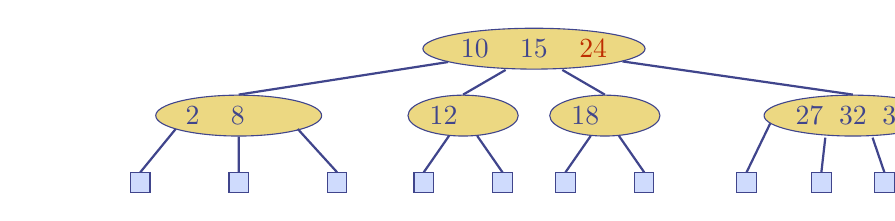
\begin{tikzpicture}[
        level 1/.style={level distance=0.85cm},
        level 2/.style={sibling distance=1cm, level distance=0.85cm},
        edge from parent/.style={draw=none},
        ]
        \hspace{1.3cm}
        \node [fath] (r) {10\hspace{0.4cm}15\hspace{0.4cm}\textcolor{naranja}{24}}
            child [sibling distance=2.5 cm] {
                node [fath] (ch1) {2\hspace{0.4cm}8\hspace{0.5cm}\textcolor{crema}{.}}
                child [sibling distance=1.25cm] {node[noneLow] (ch1a) { }}
                child [sibling distance=1.25cm] {node[noneLow] (ch1b) { }}
                child [sibling distance=1.25cm] {node[noneLow] (ch1c) { }}
            }
            child [sibling distance=1.8 cm] {
                node[fath] (ch2) {12\hspace{0.4cm}\textcolor{crema}{.}}
                child {node[noneLow] (ch2a) { }}
                child {node[noneLow] (ch2b) { }}
            }
            child [sibling distance=1.8 cm] {
                node[fath] (ch3) {18\hspace{0.4cm}\textcolor{crema}{.}}
                child {node[noneLow] (ch3a) { }}
                child {node[noneLow] (ch3b) { }}
            }
            child [sibling distance=2.7 cm] {
                node[fath] (ch4) {27\hspace{0.2cm}32\hspace{0.2cm}35}
                child [sibling distance=0.9cm] {node[noneLow] (ch4a) { }}
                child [sibling distance=0.8cm] {node[noneLow] (ch4n) { }}
                child [sibling distance=0.8cm] {node[noneLow] (ch4b) { }}
                child [sibling distance=0.9cm] {node[noneLow] (ch4c) { }}
            };

            \draw[conn] (r) -- (ch1.north);
            \draw[conn] (-0.36, -0.27) -- (ch2.north);
            \draw[conn] (0.36, -0.27) -- (ch3.north);
            \draw[conn] (r) -- (ch4.north);

            \draw[conn] (-4.55, -1.02) -- (ch1a.north);
            \draw[conn] (ch1.south) -- (ch1b.north);
            \draw[conn] (-3, -1.02) -- (ch1c.north);

            \draw[conn] (ch2) -- (ch2a.north);
            \draw[conn] (ch2) -- (ch2b.north);

            \draw[conn] (ch3) -- (ch3a.north);
            \draw[conn] (ch3) -- (ch3b.north);

            \draw[conn] (3, -0.95) -- (ch4a.north);
            \draw[conn] (3.7, -1.13) -- (ch4n.north);
            \draw[conn] (4.3, -1.13) -- (ch4b.north);
            \draw[conn] (5, -1.0) -- (ch4c.north);
    \end{tikzpicture}
    
    \hspace{6.13cm}
    \MyArrow[fill=naranja!0, draw=naranja, thick, rotate=270]{} 

    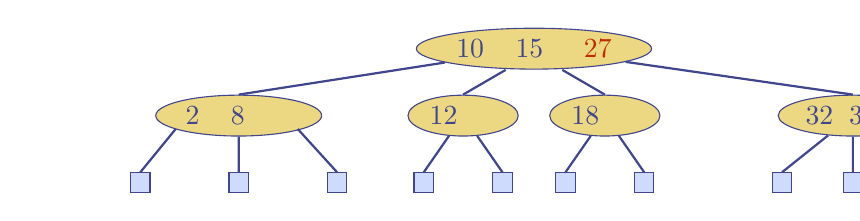
\begin{tikzpicture}[
        level 1/.style={level distance=0.85cm},
        level 2/.style={sibling distance=1cm, level distance=0.85cm},
        edge from parent/.style={draw=none},
        ]
        \hspace{1.3cm}
        \node [fath] (r) {10\hspace{0.4cm}15 \hspace{0.4cm}\textcolor{naranja}{27}}
            child [sibling distance=2.5 cm] {
                node [fath] (ch1) {2\hspace{0.4cm}8\hspace{0.5cm}\textcolor{crema}{.}}
                child [sibling distance=1.25cm] {node[noneLow] (ch1a) { }}
                child [sibling distance=1.25cm] {node[noneLow] (ch1b) { }}
                child [sibling distance=1.25cm] {node[noneLow] (ch1c) { }}
            }
            child [sibling distance= 1.8 cm] {
                node[fath] (ch2) {12\hspace{0.4cm}\textcolor{crema}{.}}
                child {node[noneLow] (ch2a) { }}
                child {node[noneLow] (ch2b) { }}
            }
            child [sibling distance= 1.8 cm] {
                node[fath] (ch3) {18\hspace{0.4cm}\textcolor{crema}{.}}
                child {node[noneLow] (ch3a) { }}
                child {node[noneLow] (ch3b) { }}
            }
            child [sibling distance=2.7 cm] {
                node[fath] (ch4) {32\hspace{0.2cm}35\hspace{0.2cm}\textcolor{crema}{.}}
                child [sibling distance=0.9cm] {node[noneLow] (ch4a) { }}
                child [sibling distance=0.8cm] {node[noneLow] (ch4b) { }}
                child [sibling distance=0.9cm] {node[noneLow] (ch4c) { }}
            };

            \draw[conn] (r) -- (ch1.north);
            \draw[conn] (-0.36, -0.27) -- (ch2.north);
            \draw[conn] (0.36, -0.27) -- (ch3.north);
            \draw[conn] (r) -- (ch4.north);

            \draw[conn] (-4.55, -1.02) -- (ch1a.north);
            \draw[conn] (ch1.south) -- (ch1b.north);
            \draw[conn] (-3, -1.02) -- (ch1c.north);

            \draw[conn] (ch2) -- (ch2a.north);
            \draw[conn] (ch2) -- (ch2b.north);

            \draw[conn] (ch3) -- (ch3a.north);
            \draw[conn] (ch3) -- (ch3b.north);

            \draw[conn] (ch4) -- (ch4a.north);
            \draw[conn] (ch4.south) -- (ch4b.north);
            \draw[conn] (ch4) -- (ch4c.north);
    \end{tikzpicture}
\end{frame}

\begin{frame}
    \frametitle{Underflow and Fusion}
    \begin{itemize} \color{purpura}
        \item[\(\diamondsuit\)] Deleting an entry from a node v may cause an \textcolor{naranja}{underflow}, where node v becomes a 1-node with one child and no keys
        \item[\(\diamondsuit\)] To handle an underflow at node \textbf{\textit{v}} with parent \textbf{\textit{u}}, we consider two cases
        \item[\(\diamondsuit\)] \textcolor{naranja}{Case 1:} the adjacent siblings of \textbf{\textit{v}} are 2-nodes
        \begin{itemize} \color{purpura}
            \item \textcolor{naranja}{Fusion operation:} we merge \textbf{\textit{v}} with an adjacent sibling \textbf{\textit{w}} and move an entry from \textbf{\textit{u}} to the merged node \textbf{\textit{v'}}

            \item After a fusion, the underflow may propagate to the parent \textbf{\textit{u}}
        \end{itemize}
    \end{itemize}

    \begin{minipage}{0.45\linewidth}
        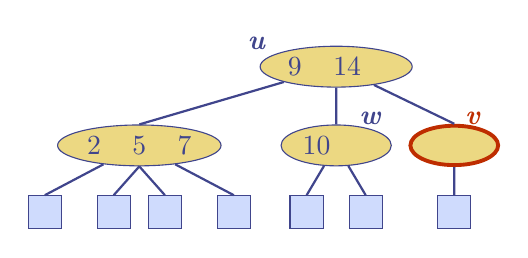
\begin{tikzpicture}[
        level 2/.style={level distance=0.85cm},
        level distance=1cm,
        edge from parent/.style={draw=none},
        ]
        \node [fath] (r) {9\hspace{0.4cm}14\hspace{0.2cm}\textcolor{crema}{.}}
            child[sibling distance=2.5cm]{
                node [fath] (ch1) {2\hspace{0.4cm}5\hspace{0.4cm}7}
                child[sibling distance=0.8cm]{node[none] (ch1a) { }}
                child[sibling distance=0.65cm]{node[none] (ch1b) { }}
                child[sibling distance=0.65cm]{node[none] (ch1c) { }}
                child[sibling distance=0.8cm]{node[none] (ch1d) { }}
            }
            child[sibling distance=2.7cm]{
                node [fath] (ch2) {10\hspace{0.4cm}\textcolor{crema}{.}}
                child[sibling distance=0.75cm]{node[none] (ch2a) { }}
                child[sibling distance=0.75cm]{node[none] (ch2b) { }}
            } 
            child[sibling distance=1.5cm]{
                node [fath, draw=naranja, line width=1.4pt, text=naranja, minimum size=0.5cm] (ch3) {\hspace{0.55cm}\textcolor{crema}{.}}
                child{node[none] (ch3a) { }}
            };

            \node[purpura] (txt1) at (-1,0.3) {\textbf{\textit{u}}};
            \node[purpura] (txt2) at (0.45,-0.65) {\textbf{\textit{w}}};
            \node[naranja] (txt3) at (1.75,-0.65) {\textbf{\textit{v}}};

            \draw[conn] (ch1.north) -- (r);
            \draw[conn] (ch2.north) -- (r);
            \draw[conn] (ch3.north) -- (r);

            \draw[conn] (ch1a.north) -- (ch1);
            \draw[conn] (ch1b.north) -- (ch1.south);
            \draw[conn] (ch1c.north) -- (ch1.south);
            \draw[conn] (ch1d.north) -- (ch1);

            \draw[conn] (ch2a.north) -- (ch2);
            \draw[conn] (ch2b.north) -- (ch2);

            \draw[conn] (ch3a.north) -- (ch3);
        \end{tikzpicture}
    \end{minipage}%
    \begin{minipage}{0.01\linewidth}
        \MyArrow[fill=naranja!0, draw=naranja, thick]{}
    \end{minipage}%
    \begin{minipage}{0.05\linewidth}
    \hspace{0.1cm}
    \end{minipage}%
    \begin{minipage}{0.45\linewidth}
        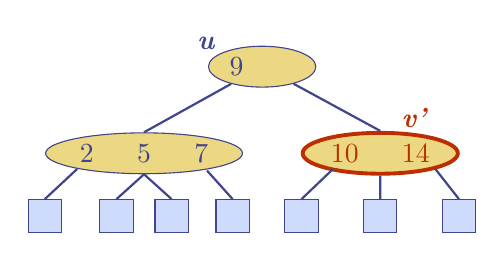
\begin{tikzpicture}[
        level 1/.style={sibling distance=3cm},
        level 2/.style={sibling distance=1cm, level distance=0.8cm},
        level 3/.style={sibling distance=1.3cm, level distance=0.8cm},
        level distance=1.1cm,
        edge from parent/.style={draw=none},
        ]
        \node [fath] (r) {9\hspace{0.55cm}\textcolor{crema}{.}}
            child {
                node [fath] (ch1) {2\hspace{0.55cm}5\hspace{0.55cm}7}
                child [sibling distance=0.84 cm] {node[none] (ch1a) { }}
                child [sibling distance=0.7 cm] {node[none] (ch1b) { }}
                child [sibling distance=0.7 cm] {node[none] (ch1c) { }}
                child [sibling distance=0.75 cm] {node[none] (ch1d) { }}
            }
            child {
                node[fath, draw=naranja, line width=1.4pt, text=naranja] (ch2) {10\hspace{0.55cm}14}
                child {node[none] (ch2a) { }}
                child {node[none] (ch2b) { }}
                child {node[none] (ch2c) { }}
            };
            
            \node[purpura] (txt1) at (-0.7,0.3) {\textbf{\textit{u}}};
            \node[naranja] (txt3) at (1.95,-0.65) {\textbf{\textit{v'}}};

            \draw[conn] (r) -- (ch1.north);
            \draw[conn] (r) -- (ch2.north);

            \draw[conn] (ch1a.north) -- (-2.35, -1.3);
            \draw[conn] (ch1b.north) -- (ch1.south);
            \draw[conn] (ch1c.north) -- (ch1.south);
            \draw[conn] (ch1d.north) -- (-0.7, -1.32);

            \draw[conn] (ch2a.north) -- (0.9, -1.3);
            \draw[conn] (ch2b.north) -- (ch2.south);
            \draw[conn] (ch2c.north) -- (2.2, -1.3);
    \end{tikzpicture}
    \end{minipage}
\end{frame}

\begin{frame}
    \frametitle{Underflow and Transfer}
    \begin{itemize} \color{purpura}
        \item[\(\diamondsuit\)] \textcolor{naranja}{Case 2:} an adjacent sibling \textbf{\textit{w}} of \textbf{\textit{v}} is a 3-node or a 4-node
        \begin{itemize} \color{purpura}
            \item \textcolor{naranja}{Transfer operation:}
            \begin{enumerate} \color{purpura}
                \item we move a child of w to v 
                \item we move an item from u to v
                \item we move an item from w to u
            \end{enumerate}
            
            \item After a fusion, the underflow may propagate to the parent \textbf{\textit{u}}
        \end{itemize}
    \end{itemize}

    \begin{minipage}{0.4\linewidth}
        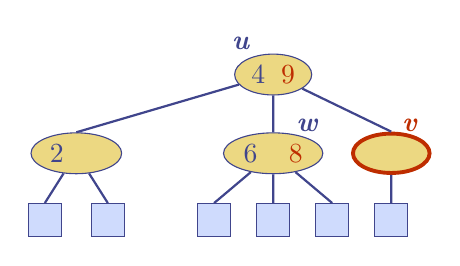
\begin{tikzpicture}[
        level 2/.style={level distance=0.85cm},
        level distance=1cm,
        edge from parent/.style={draw=none},
        ]
        \node [fath] (r) {4\hspace{0.2cm}\textcolor{naranja}{9}}
            child[sibling distance=2.5cm]{
                node [fath] (ch1) {2\hspace{0.4cm}\textcolor{crema}{.}}
                child[sibling distance=0.8cm]{node[none] (ch1a) { }}
                child[sibling distance=0.8cm]{node[none] (ch1d) { }}
            }
            child[sibling distance=2.7cm]{
                node [fath] (ch2) {6\hspace{0.4cm}\textcolor{naranja}{8}}
                child[sibling distance=0.75cm]{node[none] (ch2a) { }}
                child[sibling distance=0.75cm]{node[none] (ch2b) { }}
                child[sibling distance=0.75cm]{node[none] (ch2c) { }}
            } 
            child[sibling distance=1.5cm]{
                node [fath, draw=naranja, line width=1.4pt, text=naranja, minimum size=0.5cm] (ch3) {\hspace{0.45cm}\textcolor{crema}{.}}
                child{node[none] (ch3a) { }}
            };

            \node[purpura] (txt1) at (-0.4,0.4) {\textbf{\textit{u}}};
            \node[purpura] (txt2) at (0.45,-0.65) {\textbf{\textit{w}}};
            \node[naranja] (txt3) at (1.75,-0.65) {\textbf{\textit{v}}};

            \draw[conn] (ch1.north) -- (r);
            \draw[conn] (ch2.north) -- (r);
            \draw[conn] (ch3.north) -- (r);

            \draw[conn] (ch1a.north) -- (ch1);
            \draw[conn] (ch1d.north) -- (ch1);

            \draw[conn] (ch2a.north) -- (ch2);
            \draw[conn] (ch2b.north) -- (ch2);
            \draw[conn] (ch2c.north) -- (ch2);

            \draw[conn] (ch3a.north) -- (ch3);
        \end{tikzpicture}
    \end{minipage}%
    \begin{minipage}{0.01\linewidth}
        \MyArrow[fill=naranja!0, draw=naranja, thick]{}
    \end{minipage}%
    \begin{minipage}{0.05\linewidth}
        \hspace{0.1cm}
    \end{minipage}%
    \begin{minipage}{0.45\linewidth}
        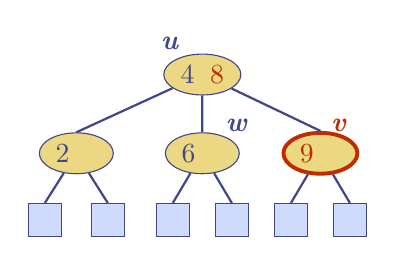
\begin{tikzpicture}[
        level 2/.style={level distance=0.85cm},
        level distance=1cm,
        edge from parent/.style={draw=none},
        ]
        \node [fath] (r) {4\hspace{0.2cm}\textcolor{naranja}{8}}
            child[sibling distance=1.6cm]{
                node [fath] (ch1) {2\hspace{0.25cm}\textcolor{crema}{.}}
                child[sibling distance=0.8cm]{node[none] (ch1a) { }}
                child[sibling distance=0.8cm]{node[none] (ch1d) { }}
            }
            child[sibling distance=1.75cm]{
                node [fath] (ch2) {6\hspace{0.25cm}\textcolor{crema}{.}}
                child[sibling distance=0.75cm]{node[none] (ch2a) { }}
                child[sibling distance=0.75cm]{node[none] (ch2b) { }}
            } 
            child[sibling distance=1.5cm]{
                node [fath, draw=naranja, line width=1.4pt, text=naranja, minimum size=0.5cm] (ch3) {\textcolor{naranja}{9}\hspace{0.25cm}\textcolor{crema}{.}}
                child[sibling distance=0.75cm]{node[none] (ch3a) { }}
                child[sibling distance=0.75cm]{node[none] (ch3b) { }}
            };

            \node[purpura] (txt1) at (-0.4,0.4) {\textbf{\textit{u}}};
            \node[purpura] (txt2) at (0.45,-0.65) {\textbf{\textit{w}}};
            \node[naranja] (txt3) at (1.75,-0.65) {\textbf{\textit{v}}};

            \draw[conn] (ch1.north) -- (r);
            \draw[conn] (ch2.north) -- (r);
            \draw[conn] (ch3.north) -- (r);

            \draw[conn] (ch1a.north) -- (ch1);
            \draw[conn] (ch1d.north) -- (ch1);

            \draw[conn] (ch2a.north) -- (ch2);
            \draw[conn] (ch2b.north) -- (ch2);

            \draw[conn] (ch3a.north) -- (ch3);
            \draw[conn] (ch3b.north) -- (ch3);
    \end{tikzpicture}
    \end{minipage}
\end{frame}

\begin{frame}
    \frametitle{Analysis of Deletion}
    \begin{itemize} \color{purpura}
        \item[\(\diamondsuit\)] Let \textbf{\textit{T}} be a (2,4) tree with \textbf{\textit{n}} items
        \begin{itemize} \color{purpura}
            \item Tree \textbf{\textit{T}} has \textbf{\textit{O}}(log \textbf{\textit{n}}) height
        \end{itemize}
        
        \item[\(\diamondsuit\)] In a delete operation
        \begin{itemize} \color{purpura}
            \item We visit \textbf{\textit{O}}(log \textbf{\textit{n}}) nodes to locate the node from which to delete the entry
            \item We handle an underflow with a series of \textbf{\textit{O}}(log \textbf{\textit{n}}) fusions, followed by at most one transfer
            \item Each fusion and transfer takes \textbf{\textit{O}}(1) time
        \end{itemize}

        \item[\(\diamondsuit\)] Thus, deleting an item from a (2,4) tree takes \textbf{\textit{O}}(log \textbf{\textit{n}}) time
    \end{itemize}
\end{frame}

\begin{frame}
    \frametitle{Comparison of Map Implementations}
% Please add the following required packages to your document preamble:
% \usepackage[table,xcdraw]{xcolor}
% Beamer presentation requires \usepackage{colortbl} instead of \usepackage[table,xcdraw]{xcolor}
\begin{table}[]
\begin{tabular}{|c|c|c|c|l|}
\hline
\rowcolor{tablepurpura} 
                                                                                      & {\color{naranja} Find}                                                       & {\color{naranja} Put}                                                        & {\color{naranja} Erase}                                                      & {\color{naranja} Notes}                                                                                  \\ \hline
\rowcolor{tablecrema} 
{\color{purpura} \begin{tabular}[c]{@{}c@{}}Hash\\ Table\end{tabular}}           & {\color{purpura} \begin{tabular}[c]{@{}c@{}}1\\ expected\end{tabular}}       & {\color{purpura} \begin{tabular}[c]{@{}c@{}}1 \\ expected\end{tabular}}      & {\color{purpura} \begin{tabular}[c]{@{}c@{}}1\\ expected\end{tabular}}       & {\color{purpura} \begin{tabular}[c]{@{}l@{}}no ordered map\\ methods\\ simple to implement\end{tabular}} \\ \hline
\rowcolor{tableamarillo} 
{\color{purpura} \begin{tabular}[c]{@{}c@{}}Skip\\ List\end{tabular}}            & {\color{purpura} \begin{tabular}[c]{@{}c@{}}log \textit{\textbf{n}}\\ high prob.\end{tabular}} & {\color{purpura} \begin{tabular}[c]{@{}c@{}}log \textbf{\textit{n}}\\ high prob.\end{tabular}} & {\color{purpura} \begin{tabular}[c]{@{}c@{}}log \textit{\textbf{n}}\\ high prob.\end{tabular}} & {\color{purpura} \begin{tabular}[c]{@{}l@{}}randomized insertion\\ simple to implement\end{tabular}}     \\ \hline
\rowcolor{celeste} 
{\color{purpura} \begin{tabular}[c]{@{}c@{}}AVL and\\ (2,4)\\ Tree\end{tabular}} & {\color{purpura} \begin{tabular}[c]{@{}c@{}}log \textbf{\textit{n}}\\ worst-case\end{tabular}} & {\color{purpura} \begin{tabular}[c]{@{}c@{}}log \textit{\textbf{n}}\\ worst-case\end{tabular}} & {\color{purpura} \begin{tabular}[c]{@{}c@{}}log \textbf{\textit{n}}\\ worst-case\end{tabular}} & {\color{purpura} complex to implement}                                                                   \\ \hline
\end{tabular}
\end{table}
    
\end{frame}

\begin{frame}
    \vspace{2cm}
    \hspace{5cm}
    \color{purpura} {\Huge \textbf{Questions?}}
\end{frame}
\end{document}